% ==========================================
% SEÇÃO 2: SÍNTESE DE CORES: RGB VS. CMYK
% ==========================================
\section{Síntese de Cores}
\begin{frame}{Síntese Aditiva: Modelo RGB}
    \begin{columns}[T]
        \begin{column}{0.55\textwidth}
            \begin{itemize}
                \item \textbf{Sistemas Aditivos de Emissão:}
                \begin{itemize}
                    \item Aplicado em hardware emissor de luz: telas OLED, LCDs, projetores e TVs.
                \end{itemize}
                \vspace{0.2cm}
                \item \textbf{Engenharia do Subpixel:}
                \begin{itemize}
                    \item Cada pixel é uma junção de emissores independentes (\textbf{R}, \textbf{G}, \textbf{B}) invisíveis a olho nu.
                \end{itemize}
                \vspace{0.2cm}
                \item \textbf{Estrutura de Memória:}
                \begin{itemize}
                    \item Representação digital direta no barramento: $C = rR + gG + bB$.
                    \item \textbf{Preto (0):} LEDs totalmente desligados.
                    \item \textbf{Branco (max):} Potência máxima nos 3 canais simultâneos.
                \end{itemize}
            \end{itemize}
        \end{column}
        
        \begin{column}{0.45\textwidth}
            \begin{figure}
                \centering
                
\includegraphics[width=0.9\textwidth]{images/sintese_aditiva_rgb.jpg}
                \caption{Sobreposição de luzes RGB.}
            \end{figure}
        \end{column}
    \end{columns}

    \note{
        \begin{columns}[T]
            \begin{column}{0.49\textwidth}
                \scriptsize

                \textbf{Foco Prático e Hardware:}
                \begin{itemize}
                    \setlength{\itemsep}{1pt}
                    \item \textbf{Aparato Físico:} Monitores projetam fótons direto no olho, diferente de uma folha que absorve e reflete luz.
                    \item \textbf{Subpixel macro:} Gota de água ou lupa na tela do celular revela os filetes isolados R, G e B acesos.
                    \item \textbf{Memória:} Na programação, pixel de 24 bits dedica 1 byte (0 a 255) para controlar a voltagem/brilho de cada lâmpada.
                    \item \textbf{Matemática Básica:} Foco no conceito: somou tudo vira Branco; cortou a energia do barramento vira Preto absoluto (telas OLED).
                \end{itemize}

                \vspace{0.1cm}
                
                Cor final é a \textbf{soma física de fótons} na retina.
            \end{column}

            \begin{column}{0.49\textwidth}    
                \scriptsize

                \textbf{O Barramento ($C = rR + gG + bB$):}
                \begin{itemize}
                    \setlength{\itemsep}{1pt}
                    \item \textbf{O que é:} Tradução exata de como o Software (seu código) controla o Hardware (os LEDs da tela).
                    \item \textbf{Fixos ($R, G, B$):} Três subpixels físicos (micro-LEDs) soldados na placa do monitor.
                    \item \textbf{Variáveis ($r, g, b$):} Valores digitais definidos na memória (ex: 0 a 255 ou 0.0 a 1.0).
                    \item \textbf{Mecanismo:} Funcionam como reguladores de voltagem. O barramento envia os números e a tela injeta corrente.
                    \item \textbf{Exemplo:} Se o código define $r=255, g=0, b=0$, manda energia máxima para o vermelho e desliga os outros, gerando vermelho puro.
                \end{itemize}
            \end{column}
        \end{columns}
    }
\end{frame}

\begin{frame}
    \begin{figure}
        \centering
        % 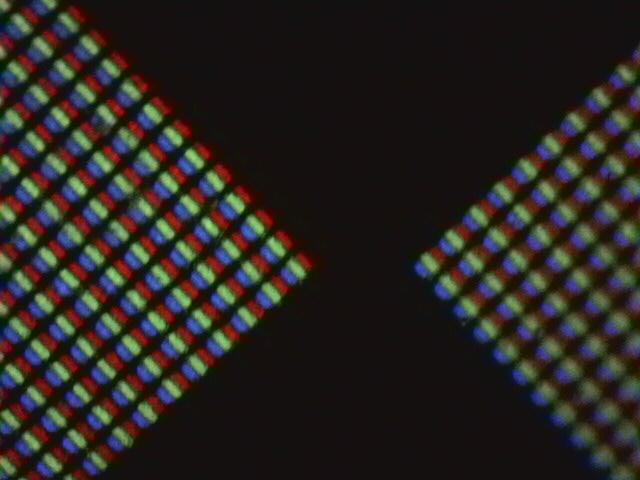
\includegraphics[width=0.9\textwidth]{images/tela_no_microscopio.jpg}
        \caption{Tela do celular ampliada no microscópio.}
    \end{figure}

    \note{
        \begin{columns}[T]
            \begin{column}{0.49\textwidth}
                \scriptsize
                \textbf{Análise da Imagem Ampliada:}
                \begin{itemize}
                    \setlength{\itemsep}{1pt}
                    \item \textbf{A Ilusão Óptica:} O que o usuário enxerga a distância como uma imagem contínua e suave, na verdade é uma matriz discreta de emissores isolados.
                    \item \textbf{Geometria do Pixel:} Cada ponto luminoso (pixel) é composto pela tríade física fixa: uma faixa Vermelha, uma Verde e uma Azul.
                    \item \textbf{Cores Secundárias:} Para gerar Amarelo, o hardware acende os filetes R e G com potência máxima e desliga o B. A mistura ocorre no espaço (retina), não na tela.
                \end{itemize}
            \end{column}

            \begin{column}{0.49\textwidth}    
                \scriptsize
                \textbf{Conexão com Baixo Nível:}
                \begin{itemize}
                    \setlength{\itemsep}{1pt}
                    \item \textbf{Controle de Intensidade:} A variação de cores que vemos na imagem não é o LED mudando de cor, mas sim a variação do brilho relativo (luminância) de cada filete.
                    \item \textbf{Densidade (PPI):} Telas modernas possuem centenas de pixels por polegada, tornando esses filetes imperceptíveis a olho nu, exigindo lentes ou macro.
                    \item \textbf{Analogia Técnica:} O Framebuffer na memória dita diretamente a modulação por largura de pulso (PWM) ou a tensão elétrica que alimenta cada um desses filetes individuais.
                \end{itemize}
            \end{column}
        \end{columns}
    }
\end{frame}

\begin{frame}{Síntese Subtrativa: Modelo CMYK}
    \begin{columns}
        \begin{column}{0.55\textwidth}
            \textbf{Sistemas Subtrativos de Absorção:}

            \begin{itemize}
                \item Aplicado em meios físicos onde a cor \textbf{não tem luz própria} (papel, tintas, corantes).
                \item A tinta funciona como um filtro: ela \textbf{subtrai (absorve)} frequências e reflete o resto.
            \end{itemize}
        \end{column}
        
        \begin{column}{0.45\textwidth}
            \begin{figure}
                \centering
                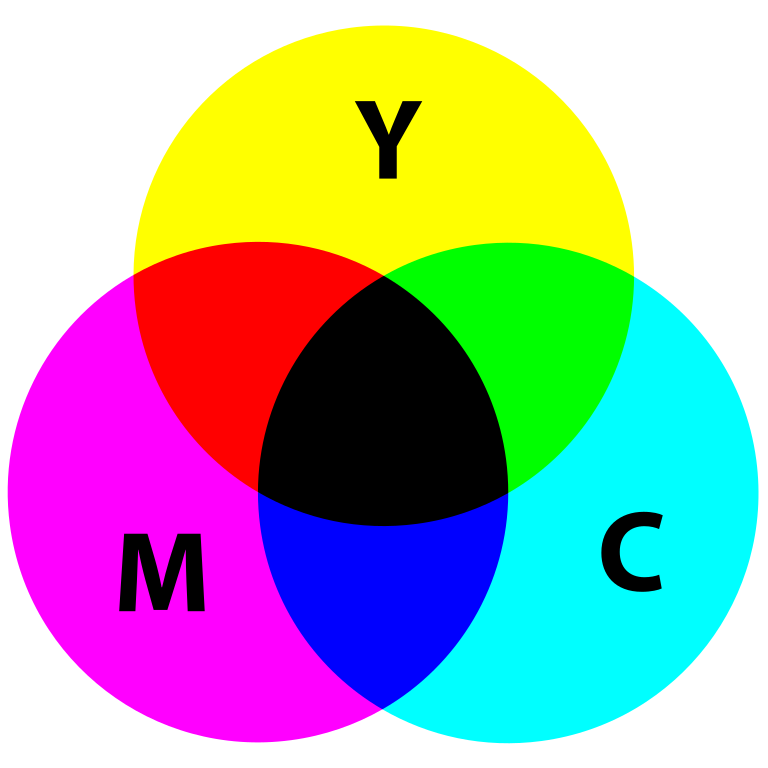
\includegraphics[width=0.9\textwidth]{images/sintese_subtrativa_cmyk.png}
                \caption{Subtração de luz - CMYK.}
            \end{figure}
        \end{column}
    \end{columns}

    \note{
        \begin{columns}[T]
            \begin{column}{0.5\textwidth}
                \scriptsize

                \textbf{Física dos Pigmentos Primários:}
                \begin{itemize}
                    \item \textbf{Ciano} absorve Vermelho (reflete G+B).
                    \item \textbf{Magenta} absorve Verde (reflete R+B).
                    \item \textbf{Amarelo} absorve Azul (reflete R+G).
                \end{itemize}

                \vspace{0.2cm}

                \textbf{A Lógica Prática:}
                \begin{itemize}
                    \setlength{\itemsep}{1pt}
                    \item \textbf{Luz Ambientes:} Para o papel ter cor, ele depende de uma luz externa (branca) batendo nele.
                    \item \textbf{O Filtro:} Quando você joga tinta ciano, você está criando uma barreira química que "engole" os fótons vermelhos da lâmpada do quarto. O que sobra e volta pro seu olho é o Verde e Azul (Ciano).
                \end{itemize}
            \end{column}

            \begin{column}{0.5\textwidth}    
                \scriptsize

                \textbf{Engenharia Gráfica:}
                \begin{itemize}
                    \setlength{\itemsep}{1pt}
                    \item \textbf{O mistério do K:} Explique que "K" vem de \textit{Key Plate} (a placa matriz preta que dava os detalhes e contornos na prensa tradicional).
                    \item \textbf{Problema de Negócio:} Se você imprimir um texto longo usando CMY para fazer preto, o papel sai molhado, enruga, rasga e a impressora gasta 3x mais cartucho. Preto puro resolve isso.
                \end{itemize}

                \textbf{Otimização de Processo (O canal K):}
                \begin{itemize}
                    \item \textbf{Engenharia Química:} Misturar $C+M+Y$ cria um marrom lamacento devido a impurezas.
                    \item \textbf{Custo e Secagem:} Usar a tinta preta ($K$) evita encharcar o papel e reduz drasticamente o custo por página.
                \end{itemize}
            \end{column}
        \end{columns}
    }
\end{frame}

\begin{frame}{O Conflito de Gamut}
    \begin{columns}[T]
        \begin{column}{0.55\textwidth}
            \begin{itemize}
                \item \textbf{O Problema do Mundo Real:}
                \begin{itemize}
                    \item \textbf{Gamut} é o limite físico de cores que um hardware consegue alcançar.
                    \item Tons "neon" ou verdes hiper-saturados do RGB dependem da emissão direta de luz. Pigmentos químicos (CMYK) não conseguem imitar esse brilho.
                \end{itemize}

                \vspace{0.2cm}

                \item \textbf{A Solução via Software:}
                \begin{itemize}
                    \item Quando uma cor da tela está "fora" do limite da impressora, o sistema roda algoritmos de \textbf{Mapeamento de Gamut}.
                \end{itemize}
            \end{itemize}
        \end{column}
        
        \begin{column}{0.45\textwidth}
            \begin{figure}
                \centering
                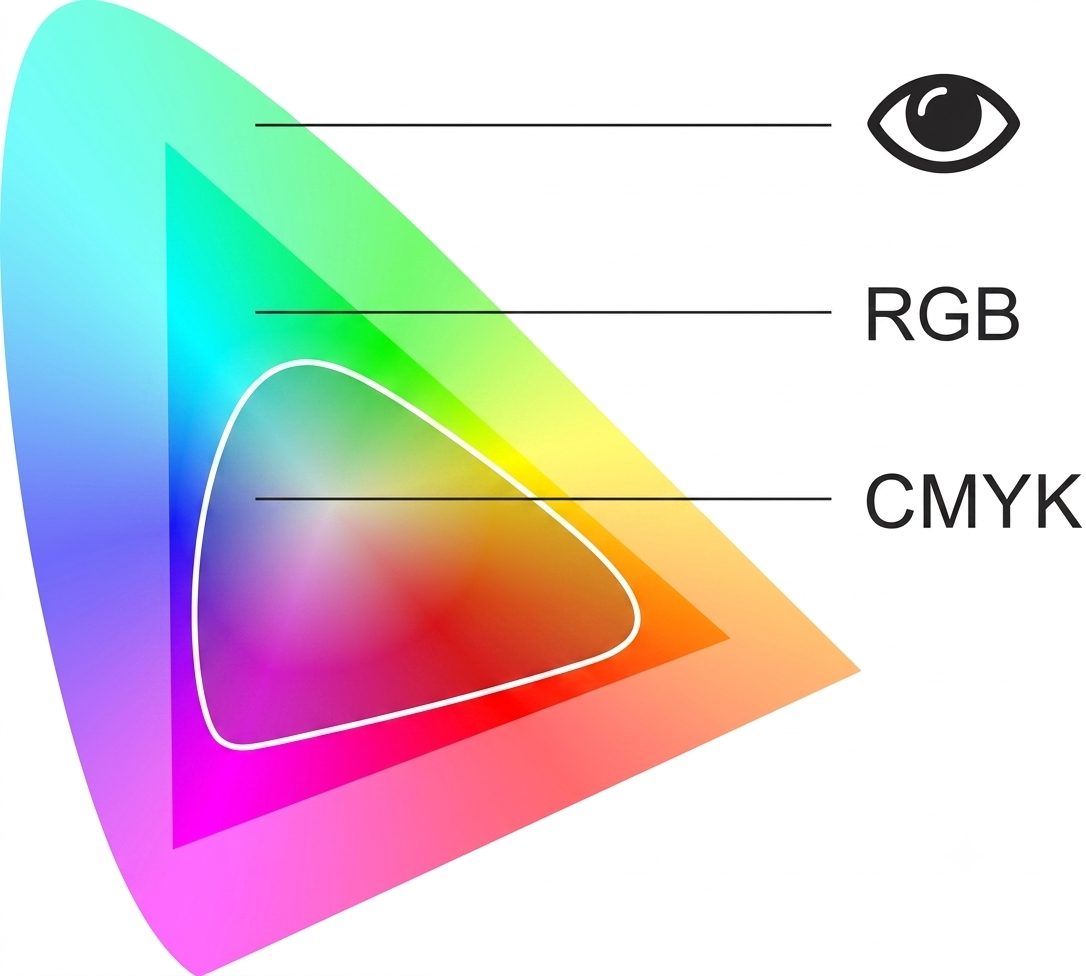
\includegraphics[width=0.9\textwidth]{images/grafico_gamut_cie.png}
                \caption{Interseção e distorção entre os limites RGB e CMYK.}
            \end{figure}
        \end{column}
    \end{columns}

    \note{
        \begin{columns}[T]
            \begin{column}{0.52\textwidth}
                \scriptsize
                \textbf{Leitura do Gráfico (Diagrama CIE):}
                \begin{itemize}
                    \setlength{\itemsep}{0pt}
                    \item \textbf{A Ferradura (Olho):} Representa todo o espectro visível pelo olho humano.
                    \item \textbf{Triângulo (RGB):} O limite que as telas alcançam. \textbf{Polígono interno (CMYK):} O limite da impressão.
                    \item \textbf{Visualização do Conflito:} A área do triângulo RGB que fica de fora do CMYK (como os verdes/azuis no topo) são as cores impossíveis de imprimir, gerando a necessidade do mapeamento.
                \end{itemize}

                \textbf{O Choque de Hardware:}
                \begin{itemize}
                    \setlength{\itemsep}{1pt}
                    \item \textbf{O Susto do Cliente:} Na tela tá um verde neon, na blusa tá um verde fosco.
                    \item \textbf{Limitação da Física:} O pigmento físico simplesmente não reflete aquela frequência de fótons.
                \end{itemize}
            \end{column}

            \begin{column}{0.48\textwidth}    
                \scriptsize
                \textbf{Estratégias de Renderização (CMS):}
                \begin{itemize}
                    \setlength{\itemsep}{1pt}
                    \item \textbf{Perceptual (Fotográfico):} Reduz o gamut inteiro proporcionalmente. Comprime todas as cores da imagem (inclusive as que a impressora conseguiria fazer) para preservar o gradiente e a relação visual entre elas. Evita estouros.
                    \item \textbf{Colorimétrico Relativo:} Faz o \textit{clipping} (poda). Mantém as cores internas idênticas e intocadas. Tudo o que estiver fora do limite é achatado (\textit{clamped}) na borda do gamut. Excelente para logos e cores sólidas exatas, mas destrói degradês finos.
                \end{itemize}
            \end{column}
        \end{columns}   
    }
\end{frame}